\documentclass[11pt]{article}

\usepackage[a4paper,margin=2.2cm]{geometry}
\usepackage[T1]{fontenc}
\usepackage{lmodern}
\usepackage{xcolor}
\usepackage{booktabs}
\usepackage{enumitem}
\usepackage{fancyhdr}
\usepackage{titlesec}
\usepackage{textcomp}
\usepackage{tikz}
\usetikzlibrary{arrows.meta,positioning}

% ---- Echo Barrier brand ----
\definecolor{ebgreen}{RGB}{2,89,69}
\definecolor{eborange}{RGB}{255,112,38}
\definecolor{ebdark}{RGB}{30,30,30}
\definecolor{ebgrey}{RGB}{107,114,128}
\definecolor{ebtint}{RGB}{237,244,242}
\definecolor{eborangetint}{RGB}{255,241,233}

\usepackage{hyperref}
\hypersetup{colorlinks=true,linkcolor=ebgreen,urlcolor=ebgreen}

\titleformat{\section}{\Large\bfseries\color{ebgreen}}{\thesection.}{0.6em}{}
\titleformat{\subsection}{\large\bfseries\color{ebdark}}{\thesubsection}{0.6em}{}
\titlespacing*{\section}{0pt}{1.4em}{0.6em}

\pagestyle{fancy}\fancyhf{}
\renewcommand{\headrulewidth}{0.6pt}
\renewcommand{\headrule}{\hbox to\headwidth{\color{ebgreen}\leaders\hrule height \headrulewidth\hfill}}
\lhead{\small\textbf{\color{ebgreen}ECHO BARRIER}}
\rhead{\small\color{ebgrey}EU AI Act --- Executive Briefing}
\cfoot{\small\color{ebgrey}\thepage}

\newcommand{\statusok}[1]{\textcolor{ebgreen}{\textbf{#1}}}
\newcommand{\statusact}[1]{\textcolor{eborange}{\textbf{#1}}}
\newcommand{\whybox}[2]{\par\vspace{4pt}\noindent\colorbox{ebtint}{\parbox{\dimexpr\linewidth-2\fboxsep}%
  {\vspace{3pt}\hspace{2pt}\textbf{\color{ebgreen}#1} #2\hspace{2pt}\vspace{3pt}}}\par\vspace{4pt}}
\newcommand{\actbox}[2]{\par\vspace{4pt}\noindent\colorbox{eborangetint}{\parbox{\dimexpr\linewidth-2\fboxsep}%
  {\vspace{3pt}\hspace{2pt}\textbf{\color{eborange}#1} #2\hspace{2pt}\vspace{3pt}}}\par\vspace{4pt}}
\setlist[itemize]{leftmargin=1.4em,itemsep=2.5pt,topsep=3pt}

\begin{document}

% =====================================================================
\noindent{\color{ebgreen}\rule{\linewidth}{2pt}}\\[0.35cm]
{\noindent\huge\bfseries\color{ebdark} The EU AI Act \& Echo Barrier}\\[0.2cm]
{\noindent\Large\color{ebgreen} Executive briefing --- what it is, where it touches us, and what we do}\\[0.25cm]
{\noindent\small\color{ebgrey} Prepared for Andy \,\textperiodcentered\, 15 July 2026 \,\textperiodcentered\, sources: Regulation (EU) 2024/1689 via \url{https://artificialintelligenceact.eu} \,\textperiodcentered\, internal --- not legal advice}\\[0.1cm]
\noindent{\color{ebgreen}\rule{\linewidth}{2pt}}

% =====================================================================
\section*{\color{ebgreen}Executive summary}

\textbf{What it is.} The EU AI Act is the EU's product-safety-style regulation of
artificial intelligence --- the first of its kind. It sorts AI systems into risk
tiers: a short list of \emph{prohibited} practices (in force since February 2025),
a heavily regulated \emph{high-risk} class (biometrics, hiring, credit, critical
infrastructure and similar), a \emph{transparency} tier for AI that talks to
people or generates content, and a \emph{minimal} tier that is effectively
unregulated. It applies to any organisation that \emph{operates} AI in the EU ---
not just to the companies that build the models. Fines scale to \texteuro 35m~/~7\%
of worldwide turnover for prohibited practices and \texteuro 15m~/~3\% for most other
breaches (SMEs pay the lower of the two figures).

\textbf{Where it applies to Echo Barrier --- and why.} Echo Barrier Group Limited
(Dublin) and Echo Barrier s.r.o.\ (Ko\v{s}ice) are EU legal entities, so wherever
the group uses AI, those entities are ``deployers'' under the Act. Our exposure is
small and manageable:

\begin{itemize}
  \item \textbf{The Hub (ERP/PO platform) is out of scope.} It is conventional,
    deterministic software --- workflows, documents, currency maths. It is not an
    AI system under the Act. \emph{No obligations attach to it.}
  \item \textbf{Echo Assist --- our AI phone assistant --- is the one deadline.}
    From \textbf{2 August 2026} (Article 50), callers must be told they are
    speaking with an AI at the start of the interaction. The fix is one line in
    the agent's greeting (English and French). This is our only date-driven item
    --- \textbf{18 days away}.
  \item \textbf{The CORTEX marketing/ops agents are minimal-risk}, provided a
    human reviews anything published --- which our ``never-post-without-approval''
    rules already enforce. We keep those gates and write them down as policy.
  \item \textbf{An obligation already in force:} since February 2025, Article 4
    requires ``AI literacy'' measures for staff who work with AI systems. A
    one-page internal guidance note and a simple register of the AI tools we
    operate satisfies this at our scale.
  \item \textbf{Nothing we run is high-risk or prohibited.} No AI makes decisions
    about people (hiring, credit, biometrics), and we do no emotion recognition
    of staff or customers.
\end{itemize}

\textbf{How we proceed.} Three low-cost actions close the gap: (1)~add the AI
disclosure line to Echo Assist \emph{before 2 August}; (2)~adopt the one-page AI
usage note + AI-systems register (Article 4); (3)~formalise the existing
human-review rule for AI-drafted public content. One adjacent flag for Corserv:
the \textbf{Section~61 platform's chat assistant} carries the same
caller/user-disclosure duty from the same date. No external counsel or tooling is
needed at our current footprint; we review the position if we ever put an AI
feature \emph{into a product we sell}.

% =====================================================================
\section{What the Act is, in one page}

\begin{center}
\begin{tabular}{@{}p{0.15\linewidth}p{0.52\linewidth}p{0.26\linewidth}@{}}
\toprule
\textbf{\color{ebgreen}Tier} & \textbf{\color{ebgreen}What falls in it} & \textbf{\color{ebgreen}Duty} \\
\midrule
Prohibited & Social scoring, manipulative AI, workplace emotion recognition, most real-time facial recognition & Banned (since Feb 2025) \\
\addlinespace
High-risk & Biometrics, hiring/HR decisions, credit, critical infrastructure, education, justice (Annex III) & Heavy: risk mgmt, documentation, oversight, conformity \\
\addlinespace
Transparency & Chatbots \& voice agents, AI-generated content, deepfakes (Article 50) & Tell people; label content \\
\addlinespace
Minimal & Everything else (most business AI) & None (voluntary codes) \\
\bottomrule
\end{tabular}
\end{center}

\vspace{0.2cm}
\noindent\textbf{Who carries duties.} \emph{Providers} (who build/sell AI) carry
the heavy obligations. \emph{Deployers} (who use AI professionally --- us) carry
lighter ones: use systems per instructions, human oversight, the transparency
duties above, and staff AI literacy. Our model vendors (Anthropic, OpenAI,
ElevenLabs) carry the provider/GPAI duties --- e.g.\ machine-readable marking of
synthetic content is \emph{their} obligation, not ours, so long as we use their
tools internally rather than selling an AI system under our own name.

\vspace{0.2cm}
\begin{center}
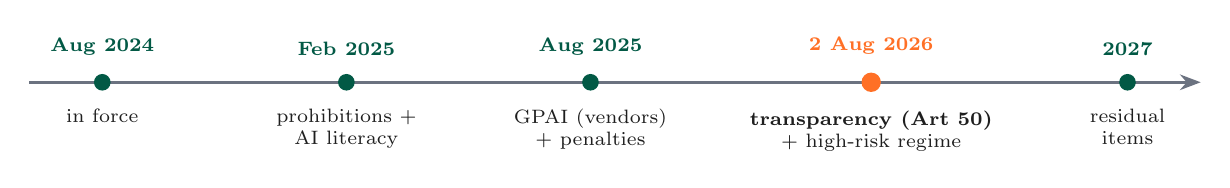
\begin{tikzpicture}[x=1.55cm,
  dot/.style={circle,fill=ebgreen,minimum size=6pt,inner sep=0pt},
  hot/.style={circle,fill=eborange,minimum size=7pt,inner sep=0pt},
  lbl/.style={font=\scriptsize,align=center,text=ebdark},
  dt/.style={font=\scriptsize\bfseries,align=center,text=ebgreen}]
\draw[line width=1pt,color=ebgrey,-{Stealth}] (0,0) -- (9.6,0);
\node[dot] (a) at (0.6,0) {}; \node[dt,above=3pt of a]{Aug 2024}; \node[lbl,below=3pt of a]{in force};
\node[dot] (b) at (2.6,0) {}; \node[dt,above=3pt of b]{Feb 2025}; \node[lbl,below=3pt of b]{prohibitions +\\AI literacy};
\node[dot] (c) at (4.6,0) {}; \node[dt,above=3pt of c]{Aug 2025}; \node[lbl,below=3pt of c]{GPAI (vendors)\\+ penalties};
\node[hot] (d) at (6.9,0) {}; \node[dt,above=3pt of d,text=eborange]{2 Aug 2026}; \node[lbl,below=3pt of d]{\textbf{transparency (Art 50)}\\+ high-risk regime};
\node[dot] (e) at (9.0,0) {}; \node[dt,above=3pt of e]{2027}; \node[lbl,below=3pt of e]{residual\\items};
\end{tikzpicture}
\end{center}

% =====================================================================
\section{Where it touches Echo Barrier --- system by system}

\begin{center}
\begin{tabular}{@{}p{0.26\linewidth}p{0.44\linewidth}p{0.20\linewidth}@{}}
\toprule
\textbf{\color{ebgreen}System} & \textbf{\color{ebgreen}Assessment} & \textbf{\color{ebgreen}Status} \\
\midrule
\textbf{The Hub} (POs, invoices, BOM, transport) & Deterministic software; not an ``AI system'' under the Act. Quote probabilities are human-entered; MRP is formula-based. & \statusok{Out of scope} \\
\addlinespace
\textbf{Echo Assist} (AI phone assistant, EN/FR) & Interacts directly with natural persons $\rightarrow$ Article 50(1): callers must be informed at first interaction that they are speaking with an AI. & \statusact{Action by 2 Aug} \\
\addlinespace
\textbf{CORTEX} (internal marketing/ops agents) & Internal deployer use = minimal risk. Published AI text only needs labelling when on ``matters of public interest'' \emph{without} human editorial review --- our human-approval gates are exactly that review. & \statusok{Keep gates; document} \\
\addlinespace
Brand / PR sentiment watchdogs & Text sentiment on public posts is not biometric ``emotion recognition''. Red line: never aim emotion inference at staff (prohibited). & \statusok{Compliant} \\
\addlinespace
High-risk screen (Annex III) & No AI making decisions about people: no hiring/credit/biometric/critical-infrastructure use. & \statusok{None present} \\
\bottomrule
\end{tabular}
\end{center}

\whybox{Why the Dublin and Ko\v{s}ice entities pull us in.}{The Act binds
\emph{deployers established in the EU} (and non-EU deployers whose system outputs
are used in the EU). Group and SRO are EU companies, so the group cannot treat
this as a UK/US question. In practice the same three actions cover every entity.}

% =====================================================================
\section{How we proceed --- the plan}

\begin{enumerate}[leftmargin=1.8em,itemsep=5pt]
  \item \textbf{Echo Assist disclosure --- before 2 August 2026.} Add one line to
    the greeting in both languages (e.g.\ ``You're speaking with Echo Barrier's
    AI assistant''). Article 50(5) requires it ``at the latest at the time of the
    first interaction''. \emph{Owner: Dean. Effort: minutes.}
  \item \textbf{Article 4 AI-literacy note + register --- this month.} A one-page
    internal note (what our AI tools are, what they may/may not be used for, that
    a human reviews anything public) plus a short register of AI systems in use
    (Echo Assist, CORTEX agents, vendor models). Already in force since Feb 2025;
    best-effort standard at our scale. \emph{Owner: Dean w/ Andy sign-off.}
  \item \textbf{Formalise the human-review rule.} The never-post-without-approval
    gates already exist in CORTEX --- one paragraph in the same note makes them
    policy, which is also our Article 50(4) carve-out for published content.
  \item \textbf{Section 61 (Corserv) --- same deadline.} Its chat assistant must
    disclose it is AI on first interaction from 2 August 2026; its noise
    calculations are deterministic and out of scope. \emph{Owner: Andy.}
  \item \textbf{Trigger for re-review.} If we ever ship an AI feature in a
    \emph{product we sell}, or use AI for decisions about people (hiring,
    credit), we reassess --- that is where provider/high-risk duties begin.
\end{enumerate}

\actbox{The one hard date:}{\textbf{2 August 2026} --- transparency obligations
apply. Everything on our list before that date is a text change or a one-page
document; nothing requires external counsel, new tooling, or budget at our
current footprint.}

\vspace{0.3cm}
\noindent{\color{ebgreen}\rule{\linewidth}{1pt}}\\[0.15cm]
\noindent{\small\color{ebgrey} Prepared from Regulation (EU) 2024/1689 as summarised at
\url{https://artificialintelligenceact.eu} (high-level summary, implementation
timeline, Articles 4, 5, 50, 99), mapped against the group's current AI estate.
Internal working document --- not legal advice; happy to walk through any item.}

\end{document}
